\documentclass[11pt,a4paper]{article}
\usepackage{manuscripts/preamble/qsd_preamble}
\usepackage{orcidlink}
\usepackage{mdframed}
\usepackage[table]{xcolor}
\usepackage{tikz}
\usetikzlibrary{arrows.meta, positioning, shapes.geometric,
                fit, backgrounds, decorations.pathreplacing}
\usepackage{booktabs}
\usepackage{array}
\geometry{margin=1in}
\hypersetup{colorlinks=true, linkcolor=blue!70!black,
  citecolor=blue!60!black, urlcolor=blue!60!black}

% --- Epistemic tag macros (local; not in qsd_preamble) ----------------------
\newcommand{\Rmark}{\textcolor{green!50!black}{\textbf{[R]}}}
\newcommand{\Cpmark}{\textcolor{blue!70!black}{\textbf{[C+]}}}
\newcommand{\Tmark}{\textcolor{orange!70!black}{\textbf{[T]}}}
\newcommand{\EXPmark}{\textcolor{red!50!black}{\textbf{[EXP]}}}
\newcommand{\Omark}{\textcolor{red!60!black}{\textbf{[O]}}}

% --- Box colour palette ------------------------------------------------------
\definecolor{Rbg}{RGB}{235,255,240}
\definecolor{Rcolor}{RGB}{40,140,60}
\definecolor{Cpbg}{RGB}{230,240,255}
\definecolor{Cpcolor}{RGB}{50,80,180}
\definecolor{Tbg}{RGB}{255,248,225}
\definecolor{Tcolor}{RGB}{160,120,20}
\definecolor{snapbg}{RGB}{255,240,240}
\definecolor{snapcol}{RGB}{180,50,50}
\definecolor{structbg}{RGB}{248,240,255}
\definecolor{structcol}{RGB}{100,40,160}
\definecolor{insightbg}{RGB}{255,248,225}
\definecolor{insightcol}{RGB}{160,120,20}
\definecolor{funnelbg}{RGB}{245,248,255}
\definecolor{lightbg}{RGB}{245,248,255}
\definecolor{axiombg}{RGB}{255,252,240}
\definecolor{axiomcol}{RGB}{180,140,40}

% --- Document-local macros ---------------------------------------------------
\newcommand{\Cq}[4]{[\![#1,#2,#3]\!]_{#4}}
\newcommand{\Ccode}[3]{[\![#1,#2,#3]\!]}
\providecommand{\Cl}[1]{\mathrm{Cl}(#1)}
\providecommand{\Hbfour}{\mathrm{Hb}_4}
\providecommand{\gs}{\varsigma}
\providecommand{\specbond}{\varpi}
\providecommand{\CL}{C_{\mathrm{L}}}
\providecommand{\Mpl}{M_{\mathrm{Pl}}}
\providecommand{\murad}{\mu_0}
\providecommand{\GN}{G_{\mathrm{N}}}
\providecommand{\Esyn}{E_{\mathrm{syn}}}
\newcommand{\nApp}{n_{\mathrm{app}}}
\newcommand{\kApp}{k_{\mathrm{app}}}

%==============================================================================
\title{%
  \textbf{Code Selection and Spacetime Signature}\\[0.5em]
  \Large How Causal Consistency, Coding Bounds, and\\
  Thermodynamic Selection Uniquely Determine\\
  $\Cq{5}{1}{3}{2}$ and $\Cl{1,3}$\\[0.8em]
  \large QSD Phase~2 --- Part~I}
\author{Marek Hubka\, \orcidlink{0009-0003-2476-9017}
  \thanks{Independent Researcher, Czech Republic.\; \\
    \href{mailto:marek@tidesofuncertainty.com}{marek@tidesofuncertainty.com}.}}
\date{\today}

\begin{document}
\maketitle

%==============================================================================
\begin{abstract}
\noindent
We derive the complete identity of the universe's quantum error-correcting code from a single axiom. Beginning with the \textbf{axiom} --- \emph{the universe is a quantum error-correcting code} $\Cq{n}{k}{d}{q}$ with all four parameters initially unknown --- we show that a two-stage elimination uniquely determines every parameter.

Stage~1 applies six sequential structural constraints. Error correction requires $d\geq3$. Causal consistency --- the absence of closed timelike curves --- forces $k=1$ via the Deutsch fixed-point mechanism, which we show is formally identical to the crossing error of any $k\geq2$ stabiliser code. The Heisenberg--Weyl group on a single qudit has rank-2 symplectic structure for every prime $q$, so there are always exactly $\tau=2$ independent error axes. Because Singleton depends only on $\tau$ and the service level $d$, it contains no $q$-dependence whatsoever; with $k=1$ and $d=3$ it gives $n=5$, and the universal native code $\Cq{5}{1}{3}{q}$ exists for every prime~$q$. Hamming saturation at $n=5$ then yields the polynomial $(q^2-1)(q^2-4)=0$, whose unique non-trivial prime solution is $q=2$. A $q=2$ observer perceiving any $\Cq{5}{1}{3}{q}$ for $q\geq3$ sees an apparent code $\Cq{\nApp}{\kApp}{3}{2}$ with $\kApp\geq6$, generating $\geq15$ CTCs --- the CTC-freedom constraint is self-reinforcing across the observer boundary.

Stage~2 is thermodynamic. The syndrome filling fraction $\Sigma(q)=(5q^2-4)/q^4$ satisfies $\Sigma(2)=1$ uniquely; all $q\geq3$ codes are thermodynamically excited states whose ghost syndrome slots dissipate $k_BT\ln 2$ per cycle by Landauer's principle.

The code's operator algebra realizes the spacetime algebra $\Cl{1,3}$ exactly --- one timelike direction carried by the single logical qubit, three spacelike directions realized in the error sector --- and the complex structure of quantum mechanics then follows geometrically, not by postulate.
\end{abstract}


\noindent\fbox{\parbox{0.97\textwidth}{%
\textbf{Epistemic Tags.}\quad
\Rmark\ rigorous within QSD;\quad
\Cpmark\ conjecture with named premise;\quad
\Tmark\ thermodynamic principle (Second Law $+$ Landauer, empirically established);\quad
\EXPmark\ exploratory / research invitation;\quad
\Omark\ open question.}}

\newpage
\tableofcontents
\newpage

%==============================================================================
\section{Introduction}
\label{sec:intro}
%==============================================================================

The universe is suspiciously stable. Isolated quantum states decohere almost immediately, yet the vacuum has maintained coherent, lawful structure for 13.8 billion years --- the same couplings, the same masses, the same physics at recombination (cosmological redshift $z\approx1100$, the epoch when the CMB formed, some 380{,}000 years after the Big Bang) as in the laboratory today. The only systems physics knows that preserve quantum information against continuous noise are error-corrected ones~\cite{Shor1995,Steane1996}. Quantum Spectrodynamics (QSD)~\cite{Hubka2026QSD} takes this observation as its starting point and proposes that the stability of physical law \emph{is} error correction: the universe is structured at the Planck scale by a quantum error-correcting code, and the constants that effective theories must measure are outputs of the code's geometry. The framework is not, specifically, a model of the Standard Model --- the SM sector is its first worked application. That original formulation showed that the $\Cq{5}{1}{3}{2}$ code reproduces all three Standard Model gauge couplings --- $\alpha^{-1}=137.033027$, $\alpha_s = 3\pi/80$, $\sin^2\theta_W = 0.231217$ --- together with the fundamental energy scale $\murad\approx 25.341$\,GeV, the Higgs mass $m_H = 5\murad \approx 126.7$\,GeV, and Newton's constant $\GN = 1/\Mpl^2$, addressing the Standard Model's $\sim$19 measured but unexplained parameters with only the Planck mass~$\Mpl$ as experimental input~\cite{Hubka2026QSD,Hubka2026QSDSupp}.

The present paper addresses the foundational question that the original formulation deferred: \emph{why this specific code?} We upgrade the axiomatic starting point from the specific code $\Cq{5}{1}{3}{2}$ to a single primitive in which every parameter is unknown:

\begin{mdframed}[backgroundcolor=axiombg,linecolor=axiomcol,
  linewidth=2pt, skipabove=8pt, skipbelow=8pt]
\textbf{QSD Axiom (L0):}\quad
\emph{The universe is a quantum error-correcting code} $\Cq{n}{k}{d}{q}$.
\end{mdframed}

\noindent
This is not a metaphor. The claim is ontological: the universe does not merely \emph{admit description by} an error-correcting code; it \emph{is} one. The four parameters $(n,k,d,q)$ --- block length, number of logical qudits, code distance, and alphabet size --- are all unknown at the outset. We derive every one of them.

The derivation proceeds in two stages. Stage~1 (Sections~\ref{sec:bounds}--\ref{sec:unique}) uses pure coding theory and causal consistency, yielding all four parameters via six sequential constraints: error correction ($d\geq3$); CTC-freedom ($k=1$, the Deutsch mechanism); $\tau=2$ universality (the rank of the symplectic form on $\mathbb{F}_q^{2n}$ is independent of $q$); Singleton blindness to $q$ (the universal native code $\Cq{5}{1}{3}{q}$ for every prime $q$); Hamming at $n=5$ (the unique solution $q=2$); observer consistency (CTC self-reinforcement). Stage~2 (Section~\ref{sec:thermo}) provides an independent thermodynamic confirmation through Landauer's principle. Section~\ref{sec:bridge} records the realization of the Clifford algebra in the code's operator algebra. Section~\ref{sec:complex} derives the complex structure of quantum mechanics. Section~\ref{sec:observer} defines the observer. Section~\ref{sec:landscape} maps the q-universe landscape. Section~\ref{sec:summary} summarises the chain Parts~II--V build upon.

%==============================================================================
\section{The Coding Bounds Landscape}
\label{sec:bounds}
%==============================================================================

Two fundamental inequalities constrain the parameters of any quantum stabiliser code $\Cq{n}{k}{d}{q}$.

The \emph{quantum Singleton bound}~\cite{KnillLaflamme1997, Rains1999} requires
\begin{equation}
  k \;\leq\; n - 2(d-1).
  \label{eq:singleton}
\end{equation}
Codes achieving equality are quantum maximum-distance separable (QMDS): they use the minimum possible syndrome overhead $n-k = 2(d-1)$ for the given distance.

The \emph{quantum Hamming bound}~\cite{Ekert1996,Gottesman1996}, for a code correcting up to $t$ errors ($d=2t+1$), requires
\begin{equation}
  q^{n-k} \;\geq\; \sum_{j=0}^{t}\binom{n}{j}(q^2-1)^j.
  \label{eq:hamming}
\end{equation}
For single-error correction ($t=1$, $d\in\{3,4\}$), this simplifies to
\begin{equation}
  q^{n-k} \;\geq\; 1 + n(q^2-1).
  \label{eq:hamming_t1}
\end{equation}
A code saturating~\eqref{eq:hamming_t1} at equality is \emph{perfect}: the $q^{n-k}$ syndrome outcomes are in exact bijection with the correctable errors, leaving no syndrome slot empty. A code that saturates \emph{both} bounds simultaneously is \emph{doubly extremal}.

\begin{mdframed}[backgroundcolor=insightbg,linecolor=insightcol, linewidth=1pt]
\textbf{Structural insight.}\quad
Double extremality is a severe constraint. A Singleton-saturating code has the minimum block length for its distance; a Hamming-saturating code has a syndrome space in perfect bijection with its error set. Demanding both simultaneously reduces the infinite space of candidate codes to a discrete --- and, as we shall see, singleton --- set.
\end{mdframed}

%==============================================================================
\section{Stage 1 --- Structural Constraints}
\label{sec:stage1}
%==============================================================================

Six sequential constraints, each logically prior to the next.

%-----------------------------------------------------------------------------
\subsection{Error correction: $d\geq3$}
\label{sec:dist}
%-----------------------------------------------------------------------------

A code with $d=1$ provides no protection: any single-qudit error corrupts the logical state irreversibly. A code with $d=2$ \emph{detects} errors but cannot \emph{correct} them --- the syndrome identifies that an error occurred but not which qudit was affected. For the code to maintain a stable logical state under continuous environmental perturbation, it must identify and correct errors. This requires $d\geq3$.

\begin{mdframed}[backgroundcolor=Rbg,linecolor=Rcolor,linewidth=1.5pt]
\textbf{Constraint~I\,\Rmark.}\quad $d\geq3$. The universe's code must correct single-qudit errors.
\end{mdframed}

%-----------------------------------------------------------------------------
\subsection{Causal consistency: $k=1$}
\label{sec:k1}
%-----------------------------------------------------------------------------

The parameter $k$ counts the number of protected logical degrees of freedom. With $k=0$ the code encodes nothing; we therefore have $k\geq1$. The more consequential constraint comes from causal consistency --- the absence of closed timelike curves (CTCs) \cite{Hawking1992, Novikov1989} --- established by the timelike structure of the logical sector together with the Deutsch fixed-point mechanism; the assembly into the spacetime algebra is given in \S\ref{sec:bridge}. Three fully worked examples for $k=1,2,6$ are deferred to Supplement~S8~\cite{Hubka2026QSDSupp}.

\paragraph{The timelike generator and the count of time directions.} The logical $Z$ operator $\bar Z$ of any stabiliser code is a Pauli string, hence $\bar Z^2 = I$. The anti-Hermitian combination $i\bar Z$ squares to $-I$:
\begin{equation}
  (i\bar Z)^2 \;=\; i^2\bar Z^2 \;=\; -I.
  \label{eq:i_zbar}
\end{equation}
The logical sector thereby supplies the candidate \emph{time-evolution generator} --- one per logical qudit. A code with $k$ logical qudits carries $k$ independent time directions. The obstruction to $k\geq2$ is geometric as well as operational: with two or more time directions, the observer split that defines the complex structure of quantum mechanics becomes circular --- mixed time--time planes generate hyperbolic rather than circular rotations, and no geometrically well-defined imaginary unit survives~\cite{Hubka2026CW}\,\Cpmark\ (named premise: quantum mechanics requires a geometrically well-defined global complex structure). The operational face of the same obstruction is exact and code-theoretic:

\paragraph{Crossing errors and the Deutsch fixed point.} A code with $k\geq2$ admits \emph{crossing errors}: stabiliser-equivalent operators that entangle pairs of logical qudits through the shared physical register. Each crossing error induces a quantum channel $M_s$ on the joint logical state, and the channel admits the Deutsch fixed-point equation~\cite{Deutsch1991}
\begin{equation}
  \rho \;=\; M_s(\rho).
  \label{eq:deutsch}
\end{equation}
The unique solution is the maximally mixed state $\rho^* = I/2^k$, from which no information can be extracted. This is the structural signature of a CTC: a self-consistent fixed point that erases every encoded bit. A code with $k\geq2$ therefore contains intrinsic CTCs at the level of its logical operators.

\paragraph{Triple equivalence.} The pathologies of $k\geq2$ are not three accidents but three faces of one structural fact:
\[
  \text{crossing error} \;\Longleftrightarrow\; \text{CTC} \;\Longleftrightarrow\; \text{ill-defined complex structure}.
\]
Only $k=1$ avoids all three. Worked-out fixed-point computations are given in Supplement~S8~\cite{Hubka2026QSDSupp}.

\begin{center}
\renewcommand{\arraystretch}{1.25}
\begin{tabular}{cccc}
\toprule
$k$ & Crossing pairs & CTCs & QM status \\
\midrule
0 & --- & --- & No time, no dynamics \\
1 & $\binom{1}{2}=0$ & 0 & \textbf{QM works} (unique $\gamma_0$-split) \\
2 & $\binom{2}{2}=1$ & 1 & Ambiguous split, QM fails \\
6 & $\binom{6}{2}=15$ & 15 & Catastrophic ($q=3$ apparent code; see \S\ref{sec:obs_ctc}) \\
\bottomrule
\end{tabular}
\end{center}

\noindent
The $k=6$ row is not a strawman: it is precisely the apparent code that a $q=2$ observer (\S\ref{sec:observer}) perceives when confronted with the native $\Cq{5}{1}{3}{3}$ code, as we derive in~\S\ref{sec:obs_ctc}.

\begin{mdframed}[backgroundcolor=Rbg,linecolor=Rcolor,linewidth=1.5pt]
\textbf{Constraint~II\,\Rmark.}\quad $k=1$. Causal consistency uniquely selects one logical qudit. The construction above maps $k$ logical qudits to $k$ timelike directions; $k\geq2$ generates crossing errors identical to CTCs via the Deutsch fixed-point mechanism~\cite{Deutsch1991}. Only $k=1$ admits a single arrow of time and a well-defined complex structure.
\end{mdframed}

%-----------------------------------------------------------------------------
\subsection{$\tau=2$ universality}
\label{sec:T2}
%-----------------------------------------------------------------------------

The next constraint is structural and universal: every prime $q$ has the same number of independent error axes per site. For a single qudit of dimension $q$, the Heisenberg--Weyl error group~\cite{Ashikhmin2001} is generated by the shift and clock operators $X_q,Z_q$ obeying $Z_qX_q = \omega X_qZ_q$ with $\omega=e^{2\pi i/q}$. Every element of the group decomposes uniquely as
\begin{equation}
  \mathcal{E}_q \;=\; \{X_q^a Z_q^b \,:\, a,b\in\mathbb{F}_q\},
  \quad |\mathcal{E}_q| \;=\; q^2.
  \label{eq:hw_basis}
\end{equation}
The $q^2-1$ non-trivial operators factor into three subsets:
\begin{equation}
  \underbrace{(q-1)}_{\text{pure }X}
  \;+\; \underbrace{(q-1)}_{\text{pure }Z}
  \;+\; \underbrace{(q-1)^2}_{\text{mixed}}
  \;=\; q^2-1.
  \label{eq:hw_count}
\end{equation}
The \emph{mixed} operators are composites $X_q^aZ_q^b$ with $a,b\neq0$; they are not independent generators but products of the two axes. This is the higher-$q$ analogue of $Y=iXZ$ in the qubit case.

The number of independent error axes $\tau$ is the rank of the symplectic form on $\mathbb{F}_q^{2n}$ that defines the stabiliser formalism. This rank is always $2$, regardless of $q$, because the symplectic structure on a one-qudit phase space is two-dimensional by construction. $\tau=2$ is therefore a topological invariant of quantum mechanics, independent of $q$. Any $q$-dependence in the bounds enters only through the cardinalities $q^2$ and $q^2-1$, never through the number of axes.

\begin{figure}[h]
\centering
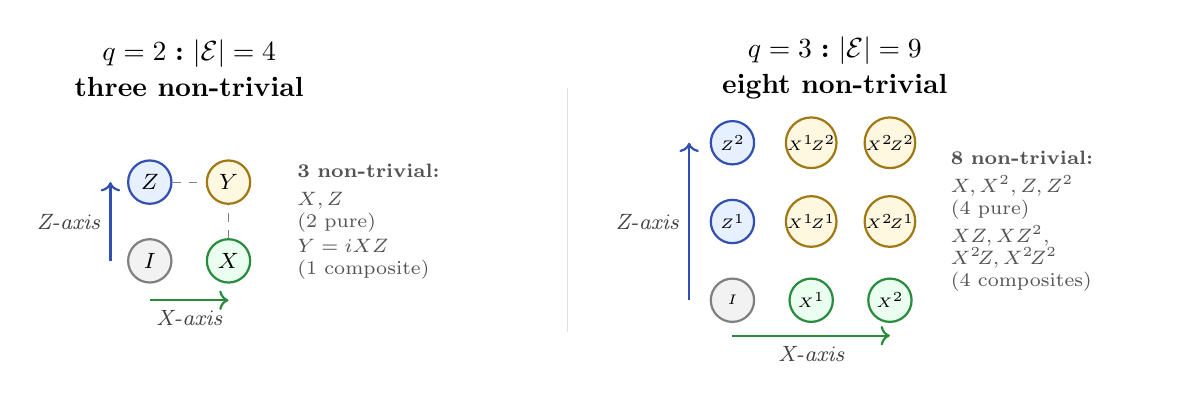
\begin{tikzpicture}[
  every node/.style={font=\footnotesize},
  op/.style={circle, draw, thick, minimum size=0.55cm, inner sep=0pt},
  pX/.style={op, fill=Rbg,       draw=Rcolor},
  pZ/.style={op, fill=Cpbg,      draw=Cpcolor},
  pM/.style={op, fill=insightbg, draw=insightcol},
  pI/.style={op, fill=gray!10,   draw=gray},
  axislab/.style={font=\footnotesize\itshape, text=gray!50!black},
  sidelab/.style={font=\scriptsize, text=gray!65!black,
                  text width=2.7cm, align=left, anchor=west}
]

%% ── LEFT: q=2 panel ─────────────────────────────────────────────
\node[font=\bfseries, align=center] at (-0.5, 3.15)
  {$q=2$\;:\;$|\mathcal{E}|=4$\\[1pt] three non-trivial};

% diagram dropped 1.5cm below title
\node[pI] (I2) at (-1.0, 0.7) {$I$};
\node[pX] (X2) at ( 0.0, 0.7) {$X$};
\node[pZ] (Z2) at (-1.0,  1.7) {$Z$};
\node[pM] (Y2) at ( 0.0,  1.7) {$Y$};

\draw[->, thick, Rcolor]  (-1.0,0.2) -- (0.0,0.2)
  node[midway, below, axislab]{X-axis};
\draw[->, thick, Cpcolor] (-1.5,0.7) -- (-1.5,1.7)
  node[midway, left,  axislab]{Z-axis};
\draw[dashed, gray] (X2) -- (Y2);
\draw[dashed, gray] (Z2) -- (Y2);

% side annotation (left panel)
\node[sidelab] at (0.75, 1.2)
  {\textbf{3 non-trivial:}\\[2pt]
   $X$,\,$Z$ \\ (2 pure)\\[1pt]
   $Y=iXZ$ \\ (1 composite)};

%% ── vertical separator ───────────────────────────
\draw[gray!25, thin] (4.3, -0.2) -- (4.3, 2.9);

%% ── RIGHT: q=3 panel ─────────────────────────────
\node[font=\bfseries, align=center] at (7.7, 3.15)
  {$q=3$\;:\;$|\mathcal{E}|=9$\\[1pt] eight non-trivial};

% 3x3 grid, dropped 1.5cm: b=0 bottom at y=-0.8
\foreach \a in {0,1,2} {
  \foreach \b in {0,1,2} {
    \pgfmathsetmacro{\xx}{6.4 + 1.0*\a}
    \pgfmathsetmacro{\yy}{0.2 + 1.0*\b}
    \ifnum\a=0
      \ifnum\b=0
        \node[pI] at (\xx,\yy) {\tiny $I$};
      \else
        \node[pZ] at (\xx,\yy) {\tiny $Z^{\b}$};
      \fi
    \else
      \ifnum\b=0
        \node[pX] at (\xx,\yy) {\tiny $X^{\a}$};
      \else
        \node[pM] at (\xx,\yy) {\tiny $X^{\a}\!Z^{\b}$};
      \fi
    \fi
  }
}

\draw[->, thick, Rcolor]  (6.4,-0.25) -- (8.4,-0.25)
  node[midway, below, axislab]{X-axis};
\draw[->, thick, Cpcolor] (5.85,0.2) -- (5.85,2.2)
  node[midway, left, axislab]{Z-axis};

% side annotation (right panel)
\node[sidelab] at (9.05, 1.2)
  {\textbf{8 non-trivial:}\\[2pt]
   $X,X^2,Z,Z^2$\\ (4 pure)\\[2pt]
   $XZ,XZ^2,$\\ $X^2\!Z,X^2\!Z^2$\\ (4 composites)};

\end{tikzpicture}
\caption{$\tau=2$ universality. Left: $q=2$, three non-trivial Pauli
operators; $Y=iXZ$ is the single composite. Right: $q=3$, eight
non-trivial operators with four pure and four composites filling the
grid interior. Independent generator axes: always two.}
\label{fig:T2}
\end{figure}

%-----------------------------------------------------------------------------
\subsection{Singleton is blind to $q$ --- the universal native code}
\label{sec:singleton_blind}
%-----------------------------------------------------------------------------

Because the Singleton bound~\eqref{eq:singleton} depends only on $\tau=2$ (through the syndrome overhead $n-k=2(d-1)$) and the service level $d$, it contains no $q$-dependence whatsoever. With $k=1$ from~\S\ref{sec:k1} and $d=3$ from~\S\ref{sec:dist},
\begin{equation}
  n \;\geq\; k + 2(d-1) \;=\; 5
  \quad \text{for every prime } q.
  \label{eq:n_5_universal}
\end{equation}
Taking the minimum at equality, $n=5$, the code $\Cq{5}{1}{3}{q}$ is a valid stabiliser code for every prime $q$. The four-stabiliser count $n-k=4$ is a universal invariant of the QSD code family.

\begin{center}
\renewcommand{\arraystretch}{1.25}
\begin{tabular}{lccc}
\toprule
Regime & $T$ & Singleton at $d=3,\,k=1$ & $n_{\min}$ \\
\midrule
Classical & 1 & $n\geq k+(d-1)$ & 3 \\
Quantum (any prime $q$) & 2 & $n\geq k+2(d-1)$ & \textbf{5} \\
\bottomrule
\end{tabular}
\end{center}

This is the \emph{universal native code landscape}. Singleton has fixed the geometry. The alphabet $q$ remains free.

\begin{figure}[h]
\centering
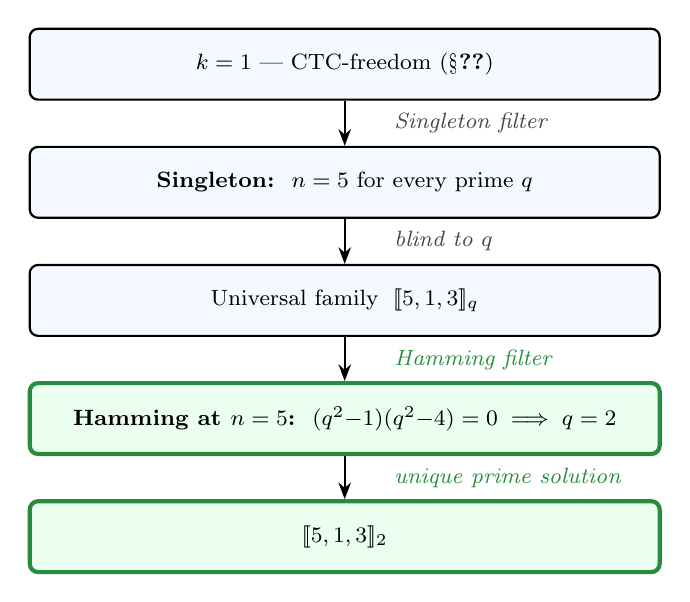
\begin{tikzpicture}[
  every node/.style={font=\footnotesize},
  box/.style={draw, rounded corners=3pt, minimum height=0.9cm,
              minimum width=8cm, align=center, thick},
  arrow/.style={-{Stealth[length=6pt]}, thick},
  sidenote/.style={font=\footnotesize\itshape, text=gray!55!black,
                   anchor=west}
]
  % vertical cascade, top -> bottom
  \node[box, fill=funnelbg] (k1) at (0, 5.0)
    {\(k=1\) --- CTC-freedom (\S\ref{sec:k1})};
  \node[box, fill=funnelbg] (sing) at (0, 3.5)
    {\textbf{Singleton:}\; $n=5$ for every prime $q$};
  \node[box, fill=funnelbg] (univ) at (0, 2.0)
    {Universal family\; $\Cq{5}{1}{3}{q}$};
  \node[box, fill=Rbg, draw=Rcolor, line width=1.5pt] (q2) at (0, 0.5)
    {\textbf{Hamming at $n=5$:}\;
     $(q^2{-}1)(q^2{-}4)=0\;\Longrightarrow\;q=2$};
  \node[box, fill=Rbg, draw=Rcolor, line width=1.5pt] (final) at (0, -1.0)
    {$\Cq{5}{1}{3}{2}$};

  % vertical arrows with side labels
  \draw[arrow] (k1)   -- (sing)
    node[sidenote] at (0.5, 4.25) {Singleton filter};
  \draw[arrow] (sing) -- (univ)
    node[sidenote] at (0.5, 2.75) {blind to $ q$};
  \draw[arrow] (univ) -- (q2)
    node[sidenote, text=Rcolor] at (0.5, 1.25) {Hamming filter};
  \draw[arrow] (q2)   -- (final)
    node[sidenote, text=Rcolor] at (0.5, -0.25) {unique prime solution};
\end{tikzpicture}
\caption{The two bounds act as sequential filters, applied top to
bottom. Singleton is blind to~$q$ and fixes the geometry $n{=}5$ for
every prime~$q$ (the universal native code $\Cq{5}{1}{3}{q}$); Hamming
then selects the alphabet $q=2$, yielding the final code
$\Cq{5}{1}{3}{2}$.}
\label{fig:filters}
\end{figure}

\begin{mdframed}[backgroundcolor=Rbg,linecolor=Rcolor,linewidth=1.5pt]
\textbf{Universal native code\,\Rmark.}\quad For every prime $q$, the
unique minimal CTC-free single-error-correcting stabiliser code is
$\Cq{5}{1}{3}{q}$. The four-stabiliser count $n-k=4$ is a universal
invariant. What varies with $q$ is not the geometry but the richness of
each syndrome measurement and the packing efficiency of the syndrome
space.
\end{mdframed}

%-----------------------------------------------------------------------------
\subsection{Hamming at $n=5$ selects $q=2$}
\label{sec:hamming_select}
%-----------------------------------------------------------------------------

With $n=5$, $k=1$, $d=3$ fixed by Singleton at the universal minimum, the Hamming bound~\eqref{eq:hamming_t1} at equality becomes
\begin{equation}
  q^4 \;=\; 1 + 5(q^2-1)
  \;\Longrightarrow\;
  q^4 - 5q^2 + 4 \;=\; (q^2-1)(q^2-4) \;=\; 0.
  \label{eq:factor}
\end{equation}
The roots are $q^2=1$ (non-physical: an alphabet of size 1 encodes nothing) and $q^2=4$, giving $\boldsymbol{q=2}$. This is the \emph{unique} prime-power solution.

The factorisation $(q^2-1)(q^2-4)$ is the arithmetic signature of double extremality at $d=3$: the factor $(q^2-4)$ is sharp at $q=2$. No other prime is permitted by Hamming saturation at $n=5$.

\paragraph{What about $d\geq4$?} The Hamming bound also constrains larger distances:

\begin{itemize}\setlength\itemsep{2pt}
\item For $d=4$, Singleton at $k=1$ gives $n=7$, $t=1$, and~\eqref{eq:hamming_t1} becomes $q^6 - 7q^2 + 6 = 0$. Checking small primes: $q=2$ gives $64-28+6=42\neq0$; $q=3$ gives $729-63+6=672\neq0$. For $q\geq4$, $q^6\gg 7q^2$. \emph{No prime-power solution exists}.
\item For $d=5$, Singleton gives $n=9$ and now $t=2$. The Hamming bound includes a second binomial term, $1+9(q^2-1)+\binom{9}{2}(q^2-1)^2 = 36q^4-63q^2+28$. At $q=2$ this evaluates to $352$, but the syndrome capacity is only $q^8=256$. The Hamming bound is not unsaturated---it is \emph{violated}: the code does not have enough syndrome space to correct all weight-$2$ errors.
\item For $d\geq6$, the Hamming gap widens monotonically with $d$ at every prime~$q$.
\end{itemize}

\begin{center}
\renewcommand{\arraystretch}{1.25}
\begin{tabular}{cccccl}
\toprule
$d$ & $n$ & $t$ & Hamming equation at $k=1$ & $q=2$ check & Outcome \\
\midrule
$3$ & $5$ & $1$ & $(q^2-1)(q^2-4)=0$ & $\checkmark$ & \textbf{Saturated} \\
$4$ & $7$ & $1$ & $q^6-7q^2+6=0$ & $42\neq0$ & No prime solution \\
$5$ & $9$ & $2$ & $q^8 = 36q^4-63q^2+28$ & $256<352$ & Violated \\
$\geq 6$ & $\geq 11$ & $\geq 2$ & --- & --- & Violated \\
\bottomrule
\end{tabular}
\end{center}

Both $d=3$ and $q=2$ are derived consequences of double extremality given $k=1$, not independent assumptions.

\begin{mdframed}[backgroundcolor=Rbg,linecolor=Rcolor,linewidth=1.5pt]
\textbf{Hamming filter\,\Rmark.}\quad At $n=5$, $k=1$, the Hamming bound at equality yields $(q^2-1)(q^2-4)=0$ with unique prime-power solution $q=2$. For all $d\geq4$, no prime-power solution exists. Both $d=3$ and $q=2$ are derived consequences of double extremality given $k=1$.
\end{mdframed}

%-----------------------------------------------------------------------------
\subsection{Observer consistency --- CTC self-reinforcement}
\label{sec:obs_ctc}
%-----------------------------------------------------------------------------

We have shown algebraically that $q=2$ is the unique Hamming-saturating alphabet. Stage~1 closes with a second, independent argument that confronts the same conclusion from a complementary angle: even without Hamming saturation, a $q\geq3$ universe would be incompatible with the CTC-freedom constraint \cite{Deutsch1991} of~\S\ref{sec:k1} once the observer is taken into account. For the QSD definition of observer used throughout, see \S\ref{sec:observer} and Supplement~S9~\cite{Hubka2026QSDSupp}.

\paragraph{Named premise.} The constraint of this subsection is~\Cpmark, with the explicit premise:
\begin{quote}
\emph{The timelike-generator and crossing construction of~\S\ref{sec:k1} extends to non-binary qudits via binary encoding}: a native $q$-ary qudit is represented in the $q=2$ Pauli algebra by $\lceil\log_2 q\rceil$ qubits, and the syndrome generators count is preserved.
\end{quote}
This premise is natural because the $\Cl{1,3}$-spacetime in which the observer lives is intrinsically $q=2$ (Constraint~II). It is~\Cpmark\ rather than~\Rmark\ because the timelike-generator and crossing analysis has been carried out in full only for $k=1$ codes; the precise statement for $k=q^2-1$ apparent qubits awaits a full proof~\Omark.

\paragraph{Apparent code under projection.} A $q=2$ observer possesses only three non-trivial single-site error operators $\{X,Z,Y=iXZ\}$. Confronted with a native $\Cq{5}{1}{3}{q}$ code for $q\geq3$, the additional $q^2-4$ error operators per site lie outside the observer's $q=2$ Pauli group. Each error dimension that is inaccessible to the observer projects out as an additional \emph{apparent} logical qubit; the four stabiliser generators remain four. Each native qudit also requires $\lceil\log_2 q\rceil$ qubits for binary representation:
\begin{equation}
  \nApp \;=\; 5\lceil\log_2 q\rceil,
  \qquad
  \kApp \;=\; \nApp - 4.
  \label{eq:apparent}
\end{equation}

For $q=3$: $\lceil\log_2 3\rceil = 2$, hence $\nApp = 10$, $\kApp = 6$, and the apparent code carries $\binom{6}{2} = 15$ crossing errors. This is precisely the $k=6$ row of the table in~\S\ref{sec:k1}---now derived rather than illustrative.

\begin{figure}[h]
\centering
\begin{tikzpicture}[
  every node/.style={font=\footnotesize},
  hdrN/.style={draw, rounded corners=3pt, fill=Rbg, draw=Rcolor,
               line width=1.2pt, minimum width=4.2cm, align=center,
               inner sep=4pt},
  hdrA/.style={draw, rounded corners=3pt, fill=Cpbg, draw=Cpcolor,
               line width=1.2pt, minimum width=4.2cm, align=center,
               inner sep=4pt},
  arr/.style={-{Stealth[length=7pt]}, thick},
  op/.style={circle, draw, thick, minimum size=0.66cm, inner sep=0pt,
             font=\tiny},
  pI/.style={op, fill=gray!12,   draw=gray},
  pX/.style={op, fill=Rbg,       draw=Rcolor},
  pZ/.style={op, fill=Cpbg,      draw=Cpcolor},
  pM/.style={op, fill=insightbg, draw=insightcol},
  % collision-partner fills for the projected grid
  cI/.style={op, fill=gray!12,   draw=gray,    dashed},
  cX/.style={op, fill=Rbg,       draw=Rcolor,  dashed},
  cZ/.style={op, fill=Cpbg,      draw=Cpcolor, dashed},
  axlab/.style={font=\tiny\itshape, text=gray!55!black}
]

%% ============ TOP ROW: code cards ============
\node[hdrN] (nat) at (0,0)
  {\textbf{Native code ($q=3$)}\\[2pt]
   $\Cq{5}{1}{3}{3}$\\[1pt]
   5 qutrits, 4 stabilisers\\
   1 logical qutrit, $d=3$};
\node[hdrA] (app) at (9.0,0)
  {\textbf{Apparent code ($q=2$ observer)}\\[2pt]
   $\Cq{10}{6}{3}{2}$\\[1pt]
   $\nApp{=}10$ qubits, 4 stabilisers\\
   $\kApp{=}6$ logical qubits, $d=3$};
\draw[arr] (nat.east) -- (app.west)
   node[midway, above, font=\footnotesize\itshape]{$q=2$ observer projection}
   node[midway, below, font=\footnotesize, text=snapcol, align=center]
      {$\binom{6}{2}=15$ CTCs\\[2pt] forbidden by~\S\ref{sec:k1}};

%% ============ BOTTOM ROW: operator grids ============
\node[font=\footnotesize\bfseries] at (0.0,-1.35)
  {$q{=}3$ native operators};
\node[font=\footnotesize\bfseries] at (9.0,-1.35)
  {projected to $q{=}2$ observer};

% ---- q=3 grid (3x3): a=col (X power) -> x, b=row (Z power) -> y up ----
\node[pI] at (-0.85,-3.80) {$I$};
\node[pX] at ( 0.00,-3.80) {$X$};
\node[pX] at ( 0.85,-3.80) {$X^2$};
\node[pZ] at (-0.85,-2.95) {$Z$};
\node[pM] at ( 0.00,-2.95) {$XZ$};
\node[pM] at ( 0.85,-2.95) {$X^{\!2}Z$};
\node[pZ] at (-0.85,-2.10) {$Z^2$};
\node[pM] at ( 0.00,-2.10) {$XZ^2$};
\node[pM] at ( 0.85,-2.10) {$X^{\!2}Z^2$};

\draw[->,thick,Rcolor]  (-0.85,-4.4)--(0.85,-4.4) node[midway, below, axlab]{X-axis};
\draw[->,thick,Cpcolor] (-1.45,-3.80)--(-1.45,-2.10) node[midway, left, axlab]{Z-axis};

% ---- projection arrow ----
\draw[arr] (2.0,-2.95) -- (6.75,-2.95)
  node[midway, above, font=\footnotesize\itshape]{$\bmod 2$ projection}
  node[midway, below, font=\tiny, text=snapcol]
    {$X^2\!\to I,\quad Z^2\!\to I$};

% ---- projected q=2 grid: same 3x3 cells, colored by collision partner ----
% accessible originals (solid):
\node[pI] at (8.15,-3.80) {$I$};
\node[pX] at (9.00,-3.80) {$X$};
\node[pZ] at (8.15,-2.95) {$Z$};
\node[pM] at (9.00,-2.95) {$XZ$};
% collisions (dashed, colored to match the partner they land on):
\node[cI] at (9.85,-3.80) {$I$};    % X^2   -> I   (gray)
\node[cZ] at (9.85,-2.95) {$IZ$};   % X^2 Z -> Z   (blue)
\node[cI] at (8.15,-2.10) {$I$};    % Z^2   -> I   (gray)
\node[cX] at (9.00,-2.10) {$XI$};   % X Z^2 -> X   (red)
\node[cI] at (9.85,-2.10) {$II$};   % X^2Z^2-> I   (gray)

% collision braces / connectors within projected grid
% \draw[gray!55, dotted, thick]   (9.85,-3.45).. controls (9.0,-3.4) ..(8.15,-3.45);     % II -> I
% \draw[Cpcolor!70, dotted, thick] (9.85,-2.95)--(8.5,-2.95);                            % IZ -> Z
% \draw[Rcolor!70, dotted, thick]  (9.00,-2.10)--(9.00,-3.45);                           % XI -> X

\node[font=\tiny, text=gray!60!black, align=center] at (9.0,-4.55)
  {dashed cells collide with their solid partner\\
   (gray$\to I$, blue$\to Z$, red$\to X$): 6 crossing errors};

\end{tikzpicture}
\caption{Observer projection. Top: a $q=2$ observer perceives the native $\Cq{5}{1}{3}{3}$ code as the apparent $\Cq{10}{6}{3}{2}$ code with six logical qubits. The $\binom{6}{2}=15$ crossing pairs are CTCs by the
Deutsch mechanism of~\S\ref{sec:k1} --- the same constraint that eliminated $k\geq2$ now eliminates $q\geq3$. Bottom: the $q=3$ Heisenberg--Weyl operator grid (left) and its $q=2$ projection (right). Under mod-2 reduction every squared factor becomes the identity, shown explicitly as frozen factors ($X^2Z\to IZ$, $XZ^2\to XI, X^2,Z^2 \to I$, and $X^2Z^2\to II$). Each projected cell is colored to match the accessible operator it collides with (gray$\to I$, blue$\to Z$, green$\to X$), making the six crossing errors visible as coincidences on the $q=2$ side.}
\label{fig:obs}
\end{figure}

The same construction at higher primes:

\begin{center}
\renewcommand{\arraystretch}{1.25}
\begin{tabular}{cccccl}
\toprule
$q$ & Native code & $\nApp$ & $\kApp$ & $\binom{\kApp}{2}$ CTCs & Status \\
\midrule
$2$ & $\Cq{5}{1}{3}{2}$ & $5$  & $1$  & $0$  & QM works \\
$3$ & $\Cq{5}{1}{3}{3}$ & $10$ & $6$  & $15$ & CTCs forbidden by~\S\ref{sec:k1} \\
$5$ & $\Cq{5}{1}{3}{5}$ & $15$ & $11$ & $55$ & CTCs forbidden by~\S\ref{sec:k1} \\
$7$ & $\Cq{5}{1}{3}{7}$ & $15$ & $11$ & $55$ & CTCs forbidden by~\S\ref{sec:k1} \\
\bottomrule
\end{tabular}
\end{center}

\noindent
\emph{The CTC-freedom constraint is self-reinforcing across the observer boundary.} The same algebraic mechanism that selected $k=1$ in~\S\ref{sec:k1} eliminates every $q\geq3$ universe for any $q=2$ observer.

\begin{mdframed}[backgroundcolor=Cpbg,linecolor=Cpcolor,linewidth=1.5pt]
\textbf{Observer consistency\,\Cpmark.}\quad
\emph{Premise:} the timelike-generator and crossing construction of~\S\ref{sec:k1} plus binary encoding of qudits. A $q=2$ observer perceiving any $\Cq{5}{1}{3}{q}$ for $q\geq3$ sees an apparent code with $\kApp\geq6$, generating at least $15$ CTCs. The CTC-freedom constraint of~\S\ref{sec:k1} eliminates $q\geq3$ for any $q=2$ observer by the same Deutsch mechanism that eliminates $k\geq2$.
\end{mdframed}

%==============================================================================
\section{The Unique Code}
\label{sec:unique}
%==============================================================================

Stage~1 has determined all four parameters from structural constraints alone, with three independent post-Hamming filters: the algebraic factorisation $(q^2-1)(q^2-4)=0$~\Rmark, the observer consistency argument~\Cpmark, and --- about to be presented in~\S\ref{sec:thermo} --- the thermodynamic ground-state argument~\Tmark. Each is sufficient on its own.

\begin{mdframed}[backgroundcolor=Rbg,linecolor=Rcolor,linewidth=2pt]
\textbf{The QECC Selection Theorem\,\Rmark.}\quad
Given L0, the code is $\Cq{5}{1}{3}{2}$. No other QECC is consistent with~L0.

\smallskip\noindent
\renewcommand{\arraystretch}{1.25}
\begin{center}
\begin{tabular}{clll}
\toprule
\textbf{Step} & \textbf{Eliminates} & \textbf{Retains} & \textbf{By} \\
\midrule
I    & $d<3$            & $d\geq3$               & Error correction \\
II   & $k=0$            & $k\geq1$               & Code encodes something \\
III  & $k\geq2$         & $k=1$                  & Deutsch CTC \\
IV   & $\tau\neq2$      & $\tau=2$               & Symplectic rank \\
V    & non-Singleton    & $n=5$                  & Blind to $q$ \\
VI   & $d\geq4$         & $d=3$                  & No Hamming solution \\
VII  & $q\neq2$         & $q=2$, $n=5$           & $(q^2-1)(q^2-4)=0$ \\
VIII & alternatives     & $\Cq{5}{1}{3}{2}$      & Gottesman--Laflamme \\
\bottomrule
\end{tabular}
\end{center}
\end{mdframed}

\noindent
Step~VIII invokes the uniqueness theorem of Gottesman~\cite{Gottesman1996} and Laflamme et al.~\cite{Laflamme1996}: among all $[\![5,1,3]\!]_2$ stabiliser codes, the cyclic-shift code is unique up to local Clifford equivalence.

\begin{figure}[h]
\centering
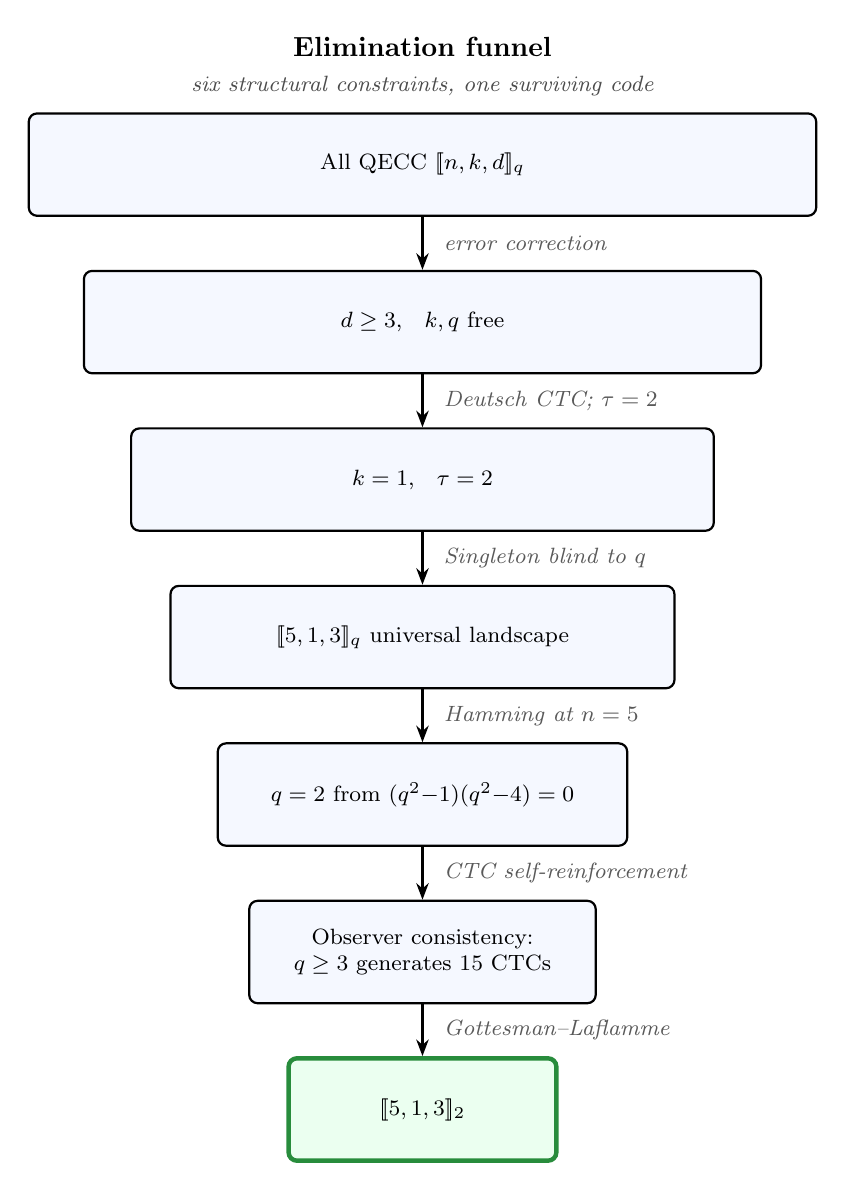
\begin{tikzpicture}[
  every node/.style={font=\footnotesize},
  box/.style={draw, rounded corners=3pt, minimum height=1.3cm,
              align=center, thick},
  arrow/.style={-{Stealth[length=6pt]}, thick},
  lbl/.style={font=\footnotesize\itshape, text=gray!70!black},
  title/.style={font=\normalsize\bfseries, text=black}
]
  \node[title] (ttl) at (0,9.5) {Elimination funnel};
  \node[font=\footnotesize\itshape, text=gray!60!black] at (0,9.0)
    {six structural constraints, one surviving code};
  \node[box, fill=funnelbg, minimum width=10cm] (all) at (0,8)
    {All QECC $\Cq{n}{k}{d}{q}$};
  \node[box, fill=funnelbg, minimum width=8.6cm] (d3) at (0,6.0)
    {$d\geq3$, \; $k,q$ free};
  \node[box, fill=funnelbg, minimum width=7.4cm] (k1) at (0,4.0)
    {$k=1$, \; $\tau=2$};
  \node[box, fill=funnelbg, minimum width=6.4cm] (sing) at (0,2.0)
    {$\Cq{5}{1}{3}{q}$ universal landscape};
  \node[box, fill=funnelbg, minimum width=5.2cm] (ham) at (0,0.0)
    {$q=2$ from $(q^2{-}1)(q^2{-}4)=0$};
  \node[box, fill=funnelbg, minimum width=4.4cm] (obs) at (0,-2.0)
    {Observer consistency: \\ $q\geq3$ generates 15 CTCs};
  \node[box, fill=Rbg, draw=Rcolor, line width=1.6pt,
        minimum width=3.4cm] (final) at (0,-4.0)
    {$\Cq{5}{1}{3}{2}$};
  \draw[arrow] (all) -- (d3) node[midway, right=4pt, lbl]{error correction};
  \draw[arrow] (d3) -- (k1) node[midway, right=4pt, lbl]{Deutsch CTC; $\tau=2$};
  \draw[arrow] (k1) -- (sing) node[midway, right=4pt, lbl]{Singleton blind to $q$};
  \draw[arrow] (sing) -- (ham) node[midway, right=4pt, lbl]{Hamming at $n=5$};
  \draw[arrow] (ham) -- (obs) node[midway, right=4pt, lbl]{CTC self-reinforcement};
  \draw[arrow] (obs) -- (final) node[midway, right=4pt, lbl]{Gottesman--Laflamme};
\end{tikzpicture}
\caption{The elimination funnel. Six structural constraints narrow the infinite landscape of QECCs to a single code. $d=3$ and $q=2$ both \emph{emerge} from the chain --- neither is assumed.}
\label{fig:funnel}
\end{figure}

\paragraph{The syndrome table.} The $n-k=4$ stabiliser generators produce $2^4=16$ syndrome patterns in exact bijection with the correctable errors: the identity plus $n(q^2-1)=5\times3=15$ weight-1 Pauli errors. The four stabiliser generators are cyclic shifts of a single string~\cite{Gottesman1996, Laflamme1996, Bennett1996}:
\begin{equation}
  S_1 \,=\, XZZXI,\quad
  S_2 \,=\, IXZZX,\quad
  S_3 \,=\, XIXZZ,\quad
  S_4 \,=\, ZXIXZ.
  \label{eq:stabilisers}
\end{equation}
The cyclic $\mathbb{Z}_5$ structure of these stabilisers is not a design choice---it is the unique solution to the constraints of~\S\ref{sec:stage1}, with downstream consequences (4-simplex geometry, $K4 \cup C5$ triad, gauge group identification) developed in Part~II.

\newpage

%==============================================================================
\section{Stage 2 --- Thermodynamic Selection}
\label{sec:thermo}
%==============================================================================

%-----------------------------------------------------------------------------
\subsection{Empirical basis}
\label{sec:thermo_empirical}
%-----------------------------------------------------------------------------

Landauer's principle and the Second Law of Thermodynamics are not axioms of QSD. They are empirically established laws of physics. The minimum energy cost to erase one bit of classical information is $k_B T \ln 2$; this was derived theoretically by Landauer~\cite{Landauer1961} and verified experimentally to within 5\% by B\'erut et al.~\cite{Berut2012} using a colloidal particle in a double-well optical trap. The Second Law itself has never been observed to be violated; for the general framework of the thermodynamics of computation see~\cite{Bennett1982}.

The epistemic tag~\Tmark---\emph{thermodynamic principle}---denotes precisely this class of claim: not an axiom of QSD, not a conjecture, but a mandatory consistency condition with experimentally established physics. A framework that violated~\Tmark\ claims would violate known thermodynamics; in this sense~\Tmark\ is structurally distinct from~\Cpmark, which records framework-internal premises whose status remains under investigation.

%-----------------------------------------------------------------------------
\subsection{The filling fraction}
\label{sec:filling_fraction}
%-----------------------------------------------------------------------------

Every error-correction cycle measures the syndrome and erases the result, incurring $k_B T \ln 2$ per syndrome bit by~\cite{Landauer1961, Berut2012}---regardless of whether the slot contains a genuine error or is empty. The relevant figure of merit is the \emph{syndrome filling fraction}: the ratio of correctable single-site error patterns to the total syndrome space.

For the universal native code $\Cq{5}{1}{3}{q}$: the syndrome space has $q^{n-k}=q^4$ patterns, the correctable set is the identity plus $5(q^2-1)$ single-site Pauli errors, and
\begin{equation}
  \Sigma(q) \;=\; \frac{1+5(q^2-1)}{q^4}
  \;=\; \frac{5q^2-4}{q^4}.
  \label{eq:Sigma}
\end{equation}
For $q=2$: $\Sigma = 16/16 = 1$. Every syndrome slot corresponds to a correctable error. The packing is perfect; no syndrome bit is wasted. For all $q\geq3$: $\Sigma<1$, decreasing as $q^{-2}$ for large~$q$. The fraction $1-\Sigma$ are \emph{ghost slots}: they must be measured and discarded each correction cycle, each dissipating $k_BT\ln2$ irreversibly. This is not engineering inefficiency; it is mandatory entropy production under the Second Law at any temperature $T>0$.

\begin{center}
\renewcommand{\arraystretch}{1.25}
\begin{tabular}{cccrl}
\toprule
$q$ & Syndrome space $q^4$ & Error patterns & $\Sigma(q)$ & Thermodynamic status \\
\midrule
$2$ & $16$   & $16$  & $100\%$ & \textbf{Ground state} \\
$3$ & $81$   & $41$  & $50.6\%$ & Excited state \\
$5$ & $625$  & $121$ & $19.4\%$ & Excited state \\
$7$ & $2401$ & $241$ & $10.0\%$ & Excited state \\
\bottomrule
\end{tabular}
\end{center}

\begin{figure}[h]
\centering
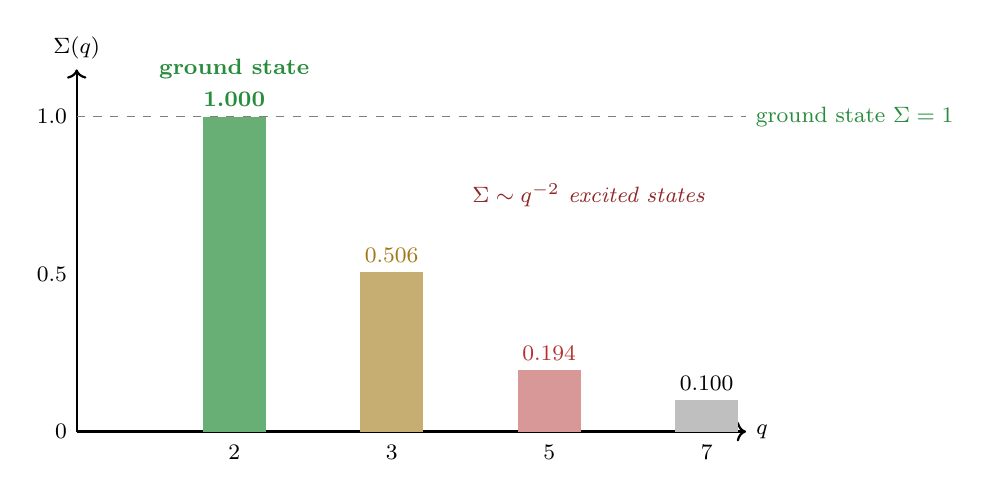
\begin{tikzpicture}[
  every node/.style={font=\footnotesize},
  axislab/.style={font=\footnotesize}
]
  % axes
  \draw[thick,->] (0,0) -- (8.5,0) node[right]{$q$};
  \draw[thick,->] (0,0) -- (0,4.6) node[above]{$\Sigma(q)$};

  % gridline at Sigma=1
  \draw[dashed, gray]  (0,4) -- (8.5,4)
    node[right, font=\footnotesize, text=Rcolor]{ground state $\Sigma=1$};
  \node[left, font=\footnotesize] at (0,4) {$1.0$};
  \node[left, font=\footnotesize] at (0,2) {$0.5$};
  \node[left, font=\footnotesize] at (0,0) {$0$};

  % bars: each at width 0.8 centered on tick
  % q=2 -> 1.0 (full bar)
  \fill[Rcolor!70]   (1.6,0)  rectangle (2.4,4.0);
  \node[above, Rcolor]   at (2.0,4.0) {\textbf{1.000}};
  \node[below]           at (2.0,-0.05) {$2$};

  % q=3 -> 0.506
  \fill[insightcol!60](3.6,0)  rectangle (4.4,2.025);
  \node[above, insightcol] at (4.0,2.025) {0.506};
  \node[below]             at (4.0,-0.05) {$3$};

  % q=5 -> 0.194
  \fill[snapcol!50]  (5.6,0)  rectangle (6.4,0.776);
  \node[above, snapcol]    at (6.0,0.776) {0.194};
  \node[below]             at (6.0,-0.05) {$5$};

  % q=7 -> 0.100
  \fill[gray!50]     (7.6,0)  rectangle (8.4,0.401);
  \node[above]             at (8.0,0.401) {0.100};
  \node[below]             at (8.0,-0.05) {$7$};

  % labels
  \node[Rcolor, font=\footnotesize\bfseries]
       at (2.0,4.6) {ground state};
  \node[snapcol!80!black, font=\footnotesize\itshape]
       at (6.5,3.0) {$\Sigma\sim q^{-2}$ excited states};
\end{tikzpicture}
\caption{Filling fraction $\Sigma(q)$ at the universal native code $\Cq{5}{1}{3}{q}$. Only $q=2$ achieves perfect syndrome packing ($\Sigma=1$). All $q\geq3$ codes carry irreducible thermodynamic overhead per correction cycle, decreasing as $q^{-2}$.}
\label{fig:sigma_q}
\end{figure}

%-----------------------------------------------------------------------------
\subsection{Ground state selection}
\label{sec:ground_state}
%-----------------------------------------------------------------------------

The codes $\Cq{5}{1}{3}{q}$ for $q\geq3$ are not incorrect: they function as valid CTC-free single-error-correcting QECCs. They are \emph{thermodynamically excited states}, carrying an irreducible entropy overhead that the $q=2$ ground state does not. At any finite temperature, a system does not remain indefinitely in an excited state when a lower-energy ground state is available---this is the operational content of the Second Law, not an additional axiom.

The $q=2$ code is the unique zero-overhead state. Stage~1 already showed it is the unique algebraic survivor; Stage~2 shows it is the unique \emph{stable} survivor in any thermal environment.

\begin{mdframed}[backgroundcolor=Tbg,linecolor=Tcolor,linewidth=1.8pt]
\textbf{Thermodynamic principle [T] --- Ground state selection.}\quad
The Second Law of Thermodynamics and Landauer's principle (both empirically established~\cite{Landauer1961, Berut2012}) require that any physical code with $\Sigma<1$ dissipates irreducible entropy per correction cycle. $\Cq{5}{1}{3}{2}$ is the unique code with $\Sigma=1$. All $q\geq3$ codes are thermodynamically excited states with irreducible overhead scaling as $q^{-2}$. This is~\Tmark: not an axiom of QSD, not a conjecture, but a mandatory consistency condition with known physics.
\end{mdframed}

%==============================================================================
\section{The Clifford Algebra --- Realization}
\label{sec:bridge}
%==============================================================================

With the code selected, this section records what the code's \emph{operator algebra} does and does not establish about the spacetime algebra $\Cl{1,3}$. The physical origin of the dimension and the signature is a hardware question and belongs to Part~II; here we stay on the software side.

\paragraph{The timelike generator.} The logical sector supplies the time-evolution generator: $\gamma_0 = i\bar Z$ squares to $-I$ by~\eqref{eq:i_zbar} and generates the phase rotation of the encoded qubit --- the $\gamma_0$-split of the algebra~\Rmark. The convention in force is the standard quantum-mechanical one --- observables Hermitian, squaring to $+I$; the time-evolution generator anti-Hermitian, squaring to $-I$ --- stated here once and used programme-wide. (The factor $i$ here is simply the scalar imaginary unit of the underlying Hilbert space; which geometric object of the algebra it represents is established in \S\ref{sec:complex}.)

\paragraph{What the operator algebra does not fix.} Neither the number of spacelike directions nor the signature is an operator-algebra fact: the five-qubit Pauli algebra contains pairwise-anticommuting sets of up to \emph{eleven} elements, and the signature of any such set is a representation convention (dressing any generator by $i$ flips its square without disturbing the anticommutation relations). Dimension and signature are fixed at the physical layer --- deferred to the hardware question of Part~II; this part makes no claim about their origin.

\paragraph{The realization.} That the code's operator algebra can \emph{carry} the resulting algebra is a theorem: an explicit generator set --- the logical operators dressed by the destabiliser sector --- reproduces the Gram matrix $\eta=\mathrm{diag}(-1,+1,+1,+1)$ exactly (exhibited in Part~II, machine-verified)~\Rmark. A framework whose code algebra could not represent $\Cl{1,3}$ would be falsified. The realization is a consistency exhibit, not an origin.

\paragraph{Pseudoscalar.} The pseudoscalar
\begin{equation}
  \mathcal{I} \;=\; \gamma_0\gamma_1\gamma_2\gamma_3
  \quad\text{satisfies}\quad
  \mathcal{I}^2 \;=\; -1
  \quad\text{in } \Cl{1,3}.
  \label{eq:I_sq}
\end{equation}
The pseudoscalar and the spatial bivectors of $\Cl{1,3}$ carry the complex structure of quantum mechanics; its geometric identification is completed in \S\ref{sec:complex}.

\begin{figure}[h]
\centering
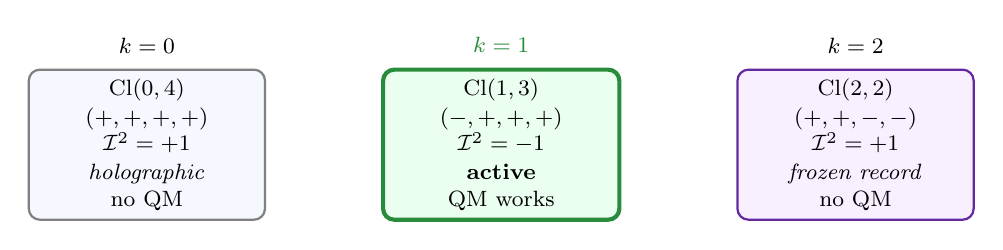
\begin{tikzpicture}[
  every node/.style={font=\footnotesize},
  phase/.style={draw, thick, rounded corners=4pt,
    minimum width=3.0cm, minimum height=1.9cm, align=center},
  arr/.style={-{Stealth[length=5pt]}, thick, gray}
]
  \node[phase, fill=lightbg, draw=gray]
        (holo) at (-4.5,0)
        {$\Cl{0,4}$\\[1pt]$(+,+,+,+)$\\$\mathcal{I}^2=+1$\\[1pt]
         \textit{holographic}\\no QM};
  \node[phase, fill=Rbg, draw=Rcolor, line width=1.5pt]
        (active) at (0,0)
        {$\boldsymbol{\Cl{1,3}}$\\[1pt]$\boldsymbol{(-,+,+,+)}$\\
         $\boldsymbol{\mathcal{I}^2=-1}$\\[1pt]
         \textbf{active}\\QM works};
  \node[phase, fill=structbg, draw=structcol]
        (frozen) at (4.5,0)
        {$\Cl{2,2}$\\[1pt]$(+,+,-,-)$\\$\mathcal{I}^2=+1$\\[1pt]
         \textit{frozen record}\\no QM};
  \node[above=2pt, font=\footnotesize\bfseries] at (holo.north) {$k=0$};
  \node[above=2pt, font=\footnotesize\bfseries, Rcolor] at (active.north) {$k=1$};
  \node[above=2pt, font=\footnotesize\bfseries] at (frozen.north) {$k=2$};
\end{tikzpicture}
\caption{The algebra family $\Cl{k,4-k}$ in context. The active phase $\Cl{1,3}$ is the unique level with $\mathcal{I}^2=-1$. The flanking algebras $\Cl{0,4}$ (holographic view) and $\Cl{2,2}$ (frozen record / ledger phase) share $\mathcal{I}^2=+1$ and do not support QM dynamics; they are information stores, treated in Parts~III and~IV. Every realized phase carries exactly four directions; $k$ only re-splits the signature.}
\label{fig:clifford_phases}
\end{figure}

\begin{mdframed}[backgroundcolor=Rbg,linecolor=Rcolor,linewidth=1.5pt]
\textbf{Clifford algebra --- realization\,\Rmark.}\quad
The code's operator algebra carries $\Cl{1,3}$ exactly: one timelike direction from the logical qubit, three spacelike directions realized in the error sector, with the explicit generator set exhibited in Part~II. What fixes the dimension and the signature physically is a hardware question, answered in Part~II. The flanking phases of the figure complete the framework's algebra family $\Cl{k,4-k}$.
\end{mdframed}

%==============================================================================
\section{The Complex Structure of Quantum Mechanics}
\label{sec:complex}
%==============================================================================

In $\Cl{1,3}$, the natural candidate for the imaginary unit of quantum mechanics is the spatial bivector
\begin{equation}
  i \;=\; \gamma_2\gamma_1.
  \label{eq:i_bivector}
\end{equation}
Both $\gamma_1$ and $\gamma_2$ are spacelike, squaring to $+I$, so
\(
  i^2 = \gamma_2\gamma_1\gamma_2\gamma_1
       = -\gamma_2^2\gamma_1^2 = -1.
\)
The pseudoscalar~\eqref{eq:I_sq} provides an alternative geometric unit and commutes with all even-grade elements; for spinor wavefunctions, the relevant unit is~\eqref{eq:i_bivector}. This is the identification established in the companion paper~\cite{Hubka2026CW}: given $\Cl{1,3}$, the Hestenes--Dirac equation, the $\gamma_0$-split, and the non-relativistic limit deliver the Schr\"odinger equation with $i$ as the projected image of the spin-plane bivector $\gamma_2\gamma_1$ --- the complex structure is a theorem of the geometry, not a postulate~\cite{Hestenes2003, Hubka2026CW}. Within QSD the chain closes without circularity: the code supplies the algebra (\S\ref{sec:bridge}, Part~II), and the geometry supplies the imaginary unit --- $i$ emerges at the \emph{end} of the chain, and nothing upstream of the algebra invokes it. That complex amplitudes are a physical necessity rather than a convention is independently supported by experiment: real-number quantum theory~\cite{Stueckelberg1960} is experimentally falsifiable~\cite{Renou2021} and has been ruled out~\cite{Chen2022}.

For any $q\geq3$ native code, no timelike generator exists at all: in the odd-$q$ Weyl--Heisenberg group the only involutions are phases --- $(\omega^a X^b Z^c)^2 = I$ forces $b\equiv c\equiv 0 \bmod q$ --- so no logical element squares to the identity and the construction of~\S\ref{sec:k1} has no seed. The Clifford structure of~\S\ref{sec:bridge} is strictly a $q=2$ phenomenon~\Rmark. This is a third independent confirmation that $q=2$ is the unique physically viable code, complementing the Hamming filter~\Rmark\ and observer consistency~\Cpmark\ of Stage~1.

The Hestenes--Dirac elaboration --- spinor structure, geometric phase, the $\bar\psi\gamma^\mu\psi$ current --- is treated in~\cite{Hestenes2003, Hubka2026CW}.

\begin{mdframed}[backgroundcolor=Rbg,linecolor=Rcolor,linewidth=1.5pt]
\textbf{Complex structure\,\Rmark.}\quad
Given the code-supplied $\Cl{1,3}$, the imaginary unit of quantum mechanics is the spin-plane bivector $\gamma_2\gamma_1$~\cite{Hubka2026CW} --- a theorem of the geometry, not a postulate. For $q\geq3$ no timelike generator can be seeded (no involutions in the odd-$q$ Weyl--Heisenberg group), so the construction itself selects $q=2$.
\end{mdframed}

\newpage

%==============================================================================
\section{The Observer}
\label{sec:observer}
%==============================================================================

The code-theoretic framework provides a precise definition of what it means to be an observer --- the question left open by the von Neumann measurement chain~\cite{vNeumannQM} and sharpened, not closed, by decoherence theory~\cite{Zurek2003}. Informally:
\begin{quote}
An \textbf{observer} is a physical system performing syndrome measurements on its environment and retaining the results in a $\Cq{n}{1}{d}{q}$ logical register. The QECC structure is not postulated --- it follows from stable memory ($d\geq3$) and definite outcomes ($k=1$ per measurement). The $q=2$ observer is the unique thermodynamically stable ground state~\Tmark\ ($\Sigma=1$).
\end{quote}
The single-logical-qubit constraint ($k=1$) ensures the observer has a well-defined arrow of time and unambiguous complex structure (Sections~\ref{sec:k1},~\ref{sec:complex}). The $q=2$ alphabet is selected by the same thermodynamic argument that selected the universe's code: a $q\geq3$ observer would itself be a thermodynamically excited state. The $q=2$ observer is therefore the unique ground-state observer; this is precisely the empirically observed situation (we are q=2 observers in a q=2 universe).

The full formal treatment, with worked syndrome-extraction examples and the asymmetry $q'$-observer $\supset$ $q$-environment, is given in Supplement~S9~\cite{Hubka2026QSDSupp}.

\begin{mdframed}[backgroundcolor=Rbg,linecolor=Rcolor,linewidth=1.5pt]
\textbf{Observer\,\Rmark.}\quad
An observer is a physical system performing syndrome measurements on its environment and retaining the results in a $\Cq{n}{1}{d}{q}$ logical register. The $q=2$ observer is the unique thermodynamically stable observer ($\Sigma=1$). Full formal treatment: Supplement~S9~\cite{Hubka2026QSDSupp}.
\end{mdframed}

%==============================================================================
\section{The q-Universe Landscape}
\label{sec:landscape}
%==============================================================================

%-----------------------------------------------------------------------------
\subsection{The universal code family}
\label{sec:univ_family}
%-----------------------------------------------------------------------------

The universal native code $\Cq{5}{1}{3}{q}$ exists for every prime~$q$ (\S\ref{sec:singleton_blind}). Each member carries an error space of per-site rank $q^2-1$. For $q=2$ this supports the realized Lorentzian algebra $\Cl{1,3}$ (\S\ref{sec:bridge}); for $q\geq3$ no timelike generator exists (\S\ref{sec:complex}), and the algebra column below is a \emph{formal count}, not a realized spacetime algebra. For each $q$, a $q=2$ observer perceives the code via the projection of~\S\ref{sec:obs_ctc}.

\begin{center}
\renewcommand{\arraystretch}{1.25}
\begin{tabular}{ccccccc}
\toprule
$q$ & Native code & Native algebra & $\nApp$ & $\kApp$ & $\Sigma(q)$ & Status \\
\midrule
$2$ & $\Cq{5}{1}{3}{2}$ & $\Cl{1,3}$  & $5$  & $1$  & $100\%$  & ground state \\
$3$ & $\Cq{5}{1}{3}{3}$ & $\Cl{1,8}$  & $10$ & $6$  & $50.6\%$ & excited \\
$5$ & $\Cq{5}{1}{3}{5}$ & $\Cl{1,24}$ & $15$ & $11$ & $19.4\%$ & excited \\
$7$ & $\Cq{5}{1}{3}{7}$ & $\Cl{1,48}$ & $15$ & $11$ & $10.0\%$ & excited \\
\bottomrule
\end{tabular}
\end{center}

The $q=2$ row's $\Cl{1,3}$ is realized (\S\ref{sec:bridge}; generator construction exhibited in Part~II)~\Rmark. The $q\geq3$ entries $\Cl{1,q^2-1}$ are formal counts only: the involution obstruction of~\S\ref{sec:complex} rules out a timelike generator for every odd prime~\Rmark, so no Lorentzian algebra is realized there. The dimensional counts $q^2-1$ themselves are direct algebraic consequences of the Heisenberg--Weyl structure and are~\Rmark.

\begin{figure}[h]
\centering
\begin{tikzpicture}[
  every node/.style={font=\footnotesize},
  level/.style ={draw, very thick, minimum width=8.5cm, minimum height=0.7cm,
                 align=center, inner sep=4pt},
  ground/.style={level, fill=Rbg, draw=Rcolor, line width=1.5pt},
  exc/.style   ={level, fill=insightbg, draw=insightcol},
  high/.style  ={level, fill=snapbg,    draw=snapcol},
  ann/.style   ={font=\footnotesize\itshape, text=gray!50!black}
]
  % axis
  \draw[->, thick] (-5.0,-0.4) -- (-5.0, 6.5) node[above]{thermodynamic energy};
  % levels: q=7 top, q=5, q=3, q=2 bottom
  \node[high]   (q7) at (0,5.5)
    {$q=7$\,: $\Cq{5}{1}{3}{7}$,\;\, $\Sigma=10.0\%$,\;\, $\kApp=11$,\;\, $\binom{11}{2}{=}55$ CTCs};
  \node[high]   (q5) at (0,4.0)
    {$q=5$\,: $\Cq{5}{1}{3}{5}$,\;\, $\Sigma=19.4\%$,\;\, $\kApp=11$,\;\, $\binom{11}{2}{=}55$ CTCs};
  \node[exc]    (q3) at (0,2.4)
    {$q=3$\,: $\Cq{5}{1}{3}{3}$,\;\, $\Sigma=50.6\%$,\;\, $\kApp=6$,\;\, $\binom{6}{2}{=}15$ CTCs};
  \node[ground] (q2) at (0,0.3)
    {$\boldsymbol{q=2}$\,: $\boldsymbol{\Cq{5}{1}{3}{2}}$,\;\, $\boldsymbol{\Sigma=100\%}$,\;\, $\boldsymbol{\kApp=1}$,\;\, \textbf{0 CTCs}};
  % ground state label
  \node[Rcolor, font=\footnotesize\bfseries] at (0.0,-0.5) {ground};
  % decay arrows
  \draw[->, dashed, gray] (q7) -- (q5);
  \draw[->, dashed, gray] (q5) -- (q3);
  \draw[->, dashed, gray] (q3) -- (q2);
  \node[ann] at (1.6,1.3) {Landauer pressure};
\end{tikzpicture}
\caption{The q-universe landscape. The family $\Cq{5}{1}{3}{q}$ for each prime $q$. Only $q=2$ is thermodynamically stable. All higher-$q$ universes are excited states with both irreducible Landauer overhead and a $q=2$-observer projection that violates CTC-freedom.}
\label{fig:landscape}
\end{figure}

%==============================================================================
\section{Summary and Outlook}
\label{sec:summary}
%==============================================================================
Starting from L0 --- the universe is a QECC $\Cq{n}{k}{d}{q}$ --- we have determined every parameter through six sequential structural constraints in Stage~1 and a thermodynamic confirmation in Stage~2. The chain of results:

\begin{center}
\renewcommand{\arraystretch}{1.25}
\begin{tabular}{ll}
\toprule
\textbf{Result} & \textbf{Status} \\
\midrule
$d\geq3$: error correction & \Rmark \\
$k=1$: CTC-freedom (Deutsch fixed point) & \Rmark \\
$\tau=2$: symplectic universality & \Rmark \\
$\Cq{5}{1}{3}{q}$: universal native code family & \Rmark \\
$q=2$: Hamming-bound unique solution & \Rmark \\
$q\geq3$: observer projection $\to$ $\geq15$ CTCs & \Cpmark \\
$q=2$: thermodynamic ground state ($\Sigma=1$) & \Tmark \\
$\Cl{1,3}$ realized in the code algebra & \Rmark \\
Complex structure: $\mathcal{I}^2=-1$ & \Rmark \\
\bottomrule
\end{tabular}
\end{center}

\noindent
\emph{No parameter is assumed.} $k=1$ is forced by causal consistency; $d=3$ and $q=2$ both emerge from the factorisation $(q^2-1)(q^2-4)=0$; $\tau=2$ is the rank of the symplectic form. The number of spatial dimensions --- three --- is a theorem, not an input.

\medskip\noindent
\textbf{What remains.}\quad
\begin{itemize}
    \item \textbf{Part~I} This part identified the code and exhibited its spacetime algebra. 
    \item \textbf{Part~II} develops the 4-simplex as a rotating object in $\Cl{1,3}$, extracts the $K4 \cup C5$ spectrum and the gauge group identification through $S_4$, derives the QSD triad ($\Hbfour, \gs, \specbond$), and computes the gauge couplings $\alpha^{-1},\,\alpha_s,\,\sin^2\theta_W$ together with the energy scale $\murad$. 
    \item \textbf{Part~III} tiles these nodes into the Bethe causal tree (branching $b=4$, coordination $z=5$) and the $\{5,4\}$ hyperbolic tessellation, derives the metric hierarchy from the K5 Gram matrix, and obtains $c=1$ in node-tick units. 
    \item \textbf{Part~IV} develops the snap as the unique structural transition, the ledger phase, the $I^2$ sandwich, the snap energy $\Esyn=\murad(1+8\gs)\approx28.24$\,GeV, the isoergic theorem, and the Big Bang as the $q\geq3\to q=2$ thermodynamic decay~\EXPmark. 
    \item \textbf{Part~V} derives the dead-node action deficit, Newtonian gravity, $\GN=1/\Mpl^2$, the Schwarzschild metric, $\gamma_{\rm PPN}=1$, and the Einstein equations $G_{\mu\nu}=8\pi\GN T_{\mu\nu}$ via Deser's uniqueness chain.
\end{itemize}

%==============================================================================

\bibliographystyle{unsrt}
\bibliography{manuscripts/references/qsd_references}

\end{document}
